% Options for packages loaded elsewhere
\PassOptionsToPackage{unicode}{hyperref}
\PassOptionsToPackage{hyphens}{url}
%
\documentclass[
  12pt,
  a4paper,
  DIV=11,
  numbers=noendperiod]{scrreprt}

\usepackage{amsmath,amssymb}
\usepackage{setspace}
\usepackage{iftex}
\ifPDFTeX
  \usepackage[T1]{fontenc}
  \usepackage[utf8]{inputenc}
  \usepackage{textcomp} % provide euro and other symbols
\else % if luatex or xetex
  \usepackage{unicode-math}
  \defaultfontfeatures{Scale=MatchLowercase}
  \defaultfontfeatures[\rmfamily]{Ligatures=TeX,Scale=1}
\fi
\usepackage{lmodern}
\ifPDFTeX\else  
    % xetex/luatex font selection
\fi
% Use upquote if available, for straight quotes in verbatim environments
\IfFileExists{upquote.sty}{\usepackage{upquote}}{}
\IfFileExists{microtype.sty}{% use microtype if available
  \usepackage[]{microtype}
  \UseMicrotypeSet[protrusion]{basicmath} % disable protrusion for tt fonts
}{}
\usepackage{xcolor}
\setlength{\emergencystretch}{3em} % prevent overfull lines
\setcounter{secnumdepth}{5}
% Make \paragraph and \subparagraph free-standing
\ifx\paragraph\undefined\else
  \let\oldparagraph\paragraph
  \renewcommand{\paragraph}[1]{\oldparagraph{#1}\mbox{}}
\fi
\ifx\subparagraph\undefined\else
  \let\oldsubparagraph\subparagraph
  \renewcommand{\subparagraph}[1]{\oldsubparagraph{#1}\mbox{}}
\fi

\usepackage{color}
\usepackage{fancyvrb}
\newcommand{\VerbBar}{|}
\newcommand{\VERB}{\Verb[commandchars=\\\{\}]}
\DefineVerbatimEnvironment{Highlighting}{Verbatim}{commandchars=\\\{\}}
% Add ',fontsize=\small' for more characters per line
\usepackage{framed}
\definecolor{shadecolor}{RGB}{241,243,245}
\newenvironment{Shaded}{\begin{snugshade}}{\end{snugshade}}
\newcommand{\AlertTok}[1]{\textcolor[rgb]{0.68,0.00,0.00}{#1}}
\newcommand{\AnnotationTok}[1]{\textcolor[rgb]{0.37,0.37,0.37}{#1}}
\newcommand{\AttributeTok}[1]{\textcolor[rgb]{0.40,0.45,0.13}{#1}}
\newcommand{\BaseNTok}[1]{\textcolor[rgb]{0.68,0.00,0.00}{#1}}
\newcommand{\BuiltInTok}[1]{\textcolor[rgb]{0.00,0.23,0.31}{#1}}
\newcommand{\CharTok}[1]{\textcolor[rgb]{0.13,0.47,0.30}{#1}}
\newcommand{\CommentTok}[1]{\textcolor[rgb]{0.37,0.37,0.37}{#1}}
\newcommand{\CommentVarTok}[1]{\textcolor[rgb]{0.37,0.37,0.37}{\textit{#1}}}
\newcommand{\ConstantTok}[1]{\textcolor[rgb]{0.56,0.35,0.01}{#1}}
\newcommand{\ControlFlowTok}[1]{\textcolor[rgb]{0.00,0.23,0.31}{#1}}
\newcommand{\DataTypeTok}[1]{\textcolor[rgb]{0.68,0.00,0.00}{#1}}
\newcommand{\DecValTok}[1]{\textcolor[rgb]{0.68,0.00,0.00}{#1}}
\newcommand{\DocumentationTok}[1]{\textcolor[rgb]{0.37,0.37,0.37}{\textit{#1}}}
\newcommand{\ErrorTok}[1]{\textcolor[rgb]{0.68,0.00,0.00}{#1}}
\newcommand{\ExtensionTok}[1]{\textcolor[rgb]{0.00,0.23,0.31}{#1}}
\newcommand{\FloatTok}[1]{\textcolor[rgb]{0.68,0.00,0.00}{#1}}
\newcommand{\FunctionTok}[1]{\textcolor[rgb]{0.28,0.35,0.67}{#1}}
\newcommand{\ImportTok}[1]{\textcolor[rgb]{0.00,0.46,0.62}{#1}}
\newcommand{\InformationTok}[1]{\textcolor[rgb]{0.37,0.37,0.37}{#1}}
\newcommand{\KeywordTok}[1]{\textcolor[rgb]{0.00,0.23,0.31}{#1}}
\newcommand{\NormalTok}[1]{\textcolor[rgb]{0.00,0.23,0.31}{#1}}
\newcommand{\OperatorTok}[1]{\textcolor[rgb]{0.37,0.37,0.37}{#1}}
\newcommand{\OtherTok}[1]{\textcolor[rgb]{0.00,0.23,0.31}{#1}}
\newcommand{\PreprocessorTok}[1]{\textcolor[rgb]{0.68,0.00,0.00}{#1}}
\newcommand{\RegionMarkerTok}[1]{\textcolor[rgb]{0.00,0.23,0.31}{#1}}
\newcommand{\SpecialCharTok}[1]{\textcolor[rgb]{0.37,0.37,0.37}{#1}}
\newcommand{\SpecialStringTok}[1]{\textcolor[rgb]{0.13,0.47,0.30}{#1}}
\newcommand{\StringTok}[1]{\textcolor[rgb]{0.13,0.47,0.30}{#1}}
\newcommand{\VariableTok}[1]{\textcolor[rgb]{0.07,0.07,0.07}{#1}}
\newcommand{\VerbatimStringTok}[1]{\textcolor[rgb]{0.13,0.47,0.30}{#1}}
\newcommand{\WarningTok}[1]{\textcolor[rgb]{0.37,0.37,0.37}{\textit{#1}}}

\providecommand{\tightlist}{%
  \setlength{\itemsep}{0pt}\setlength{\parskip}{0pt}}\usepackage{longtable,booktabs,array}
\usepackage{calc} % for calculating minipage widths
% Correct order of tables after \paragraph or \subparagraph
\usepackage{etoolbox}
\makeatletter
\patchcmd\longtable{\par}{\if@noskipsec\mbox{}\fi\par}{}{}
\makeatother
% Allow footnotes in longtable head/foot
\IfFileExists{footnotehyper.sty}{\usepackage{footnotehyper}}{\usepackage{footnote}}
\makesavenoteenv{longtable}
\usepackage{graphicx}
\makeatletter
\def\maxwidth{\ifdim\Gin@nat@width>\linewidth\linewidth\else\Gin@nat@width\fi}
\def\maxheight{\ifdim\Gin@nat@height>\textheight\textheight\else\Gin@nat@height\fi}
\makeatother
% Scale images if necessary, so that they will not overflow the page
% margins by default, and it is still possible to overwrite the defaults
% using explicit options in \includegraphics[width, height, ...]{}
\setkeys{Gin}{width=\maxwidth,height=\maxheight,keepaspectratio}
% Set default figure placement to htbp
\makeatletter
\def\fps@figure{htbp}
\makeatother

\usepackage{indentfirst}
\usepackage{float}
\floatplacement{figure}{H}
\IfFileExists{plex-otf.sty}{
  %% Full TeXlive
  \usepackage[
    % math,
    RM={Scale=0.94},SS={Scale=0.94},SScon={Scale=0.94},TT={Scale=MatchLowercase,FakeStretch=0.9},
    DefaultFeatures={Ligatures=Common}
  ]{plex-otf}
  % \usepackage[Scale=MatchUppercase]{juliamono}
}{
  %% TinyTeX
  \usepackage{libertine}
}
\KOMAoption{captions}{tableheading}
\makeatletter
\@ifpackageloaded{caption}{}{\usepackage{caption}}
\AtBeginDocument{%
\ifdefined\contentsname
  \renewcommand*\contentsname{Содержание}
\else
  \newcommand\contentsname{Содержание}
\fi
\ifdefined\listfigurename
  \renewcommand*\listfigurename{Список иллюстраций}
\else
  \newcommand\listfigurename{Список иллюстраций}
\fi
\ifdefined\listtablename
  \renewcommand*\listtablename{Список таблиц}
\else
  \newcommand\listtablename{Список таблиц}
\fi
\ifdefined\figurename
  \renewcommand*\figurename{Рисунок}
\else
  \newcommand\figurename{Рисунок}
\fi
\ifdefined\tablename
  \renewcommand*\tablename{Таблица}
\else
  \newcommand\tablename{Таблица}
\fi
}
\@ifpackageloaded{float}{}{\usepackage{float}}
\floatstyle{ruled}
\@ifundefined{c@chapter}{\newfloat{codelisting}{h}{lop}}{\newfloat{codelisting}{h}{lop}[chapter]}
\floatname{codelisting}{Список}
\newcommand*\listoflistings{\listof{codelisting}{Листинги}}
\makeatother
\makeatletter
\makeatother
\makeatletter
\@ifpackageloaded{caption}{}{\usepackage{caption}}
\@ifpackageloaded{subcaption}{}{\usepackage{subcaption}}
\makeatother
\ifLuaTeX
\usepackage[bidi=basic]{babel}
\else
\usepackage[bidi=default]{babel}
\fi
\babelprovide[main,import]{russian}
\babelprovide[import]{english}
% get rid of language-specific shorthands (see #6817):
\let\LanguageShortHands\languageshorthands
\def\languageshorthands#1{}
\ifLuaTeX
  \usepackage{selnolig}  % disable illegal ligatures
\fi
\usepackage[style=gost-numeric,backend=biber,langhook=extras,autolang=other*]{biblatex}
\addbibresource{bib/cite.bib}
\usepackage{csquotes}
\usepackage{bookmark}

\IfFileExists{xurl.sty}{\usepackage{xurl}}{} % add URL line breaks if available
\urlstyle{same} % disable monospaced font for URLs
\hypersetup{
  pdftitle={Отчёта по лабораторной работе 6},
  pdfauthor={Нджову Нелиа},
  pdflang={ru-RU},
  hidelinks,
  pdfcreator={LaTeX via pandoc}}

\title{Отчёта по лабораторной работе 6}
\usepackage{etoolbox}
\makeatletter
\providecommand{\subtitle}[1]{% add subtitle to \maketitle
  \apptocmd{\@title}{\par {\large #1 \par}}{}{}
}
\makeatother
\subtitle{Иммитационное моделирование}
\author{Нджову Нелиа}
\date{}

\begin{document}
\maketitle

\renewcommand*\contentsname{Содержание}
{
\setcounter{tocdepth}{1}
\tableofcontents
}
\listoffigures
\listoftables
\setstretch{1.5}
\chapter{Цель
работы}\label{ux446ux435ux43bux44c-ux440ux430ux431ux43eux442ux44b}

Цель этой лабораторной работы - Реализация основных моделей в подходе
сетей Петри.

\chapter{Задание}\label{ux437ux430ux434ux430ux43dux438ux435}

\begin{enumerate}
\def\labelenumi{\arabic{enumi}.}
\item
  Основная программа
\item
  Базовый прогон модели
\item
  Коэффициент заражения \(\beta\)
\item
  Анимация детерминированной динамики
\item
  Итоговый отчёт
\end{enumerate}

\chapter{Теоретическое
введение}\label{ux442ux435ux43eux440ux435ux442ux438ux447ux435ux441ux43aux43eux435-ux432ux432ux435ux434ux435ux43dux438ux435}

Реализована модель эпидемии SIR (Susceptible--Infectious--Recovered) с
использованием сетей Петри. Модель описывает переходы между тремя
состояниями:

--- S (восприимчивые) --- могут заразиться;

--- I (инфицированные) --- заражают других и выздоравливают;

--- R (выздоровевшие / с иммунитетом) --- больше не участвуют в
эпидемии.

Сеть Петри содержит два перехода:

--- infection: S + I → I + I (скорость \(\beta\)); --- recovery: I → R
(скорость \(\gamma\)).

\chapter{Выполнение лабораторной
работы}\label{ux432ux44bux43fux43eux43bux43dux435ux43dux438ux435-ux43bux430ux431ux43eux440ux430ux442ux43eux440ux43dux43eux439-ux440ux430ux431ux43eux442ux44b}

\section{1. Основная
программа}\label{ux43eux441ux43dux43eux432ux43dux430ux44f-ux43fux440ux43eux433ux440ux430ux43cux43cux430}

Я создала файл src/SIRPetri.jl и скопировала заданный скрипт в него.
Скрипт реализует вычислительную логику модели. Скрипт содержатся
несколько основые функции. Функция build\_sir\_network для построения
сети Петри, функция simulate\_deterministic для детерминированной
симуляции, функция simulate\_stochastic для стохастической симуляции,
функция sir\_ode для вспомогательной функция ОДУ, функция для
визуализации и функция для визуализации сети Петри. Я запускала и все
работала хорошо(рис.1)

\begin{figure}

\centering{


\includegraphics[width=0.7\textwidth,height=\textheight]{image/pic1.png}

}

\caption{\label{fig-001}Основная программа}

\end{figure}%

\section{2. Базовый прогон
модели}\label{ux431ux430ux437ux43eux432ux44bux439-ux43fux440ux43eux433ux43eux43d-ux43cux43eux434ux435ux43bux438}

Я создала фаий scripts/sirpetri\_run.jl и скопировала заданный скрипт в
него. Скрипт выполняет один базовый эксперимент с фиксированными
параметрами β = 0.3, γ = 0.1, запуская два типа симуляции:
детерминированную (решение ОДУ) и стохастическую (алгоритм Гиллеспи). Я
преобразовала скрипт в литератуный стиль и запускала его(рис.2)

\begin{figure}

\centering{


\includegraphics[width=0.7\textwidth,height=\textheight]{image/pic2.png}

}

\caption{\label{fig-002}Скрипт базового эксперимент}

\end{figure}%

После запуск, получила два графика. Детерминированный график показывает
классический пик эпидемии: рост I максимум, затем спад до нуля; R растёт
и выходит на плато, S падает. Стохастический график может иметь шумы и,
возможно, немного отличаться по времени пика и амплитуде -- это
демонстрирует влияние случайности(рис 3 и 4)

\begin{figure}

\centering{

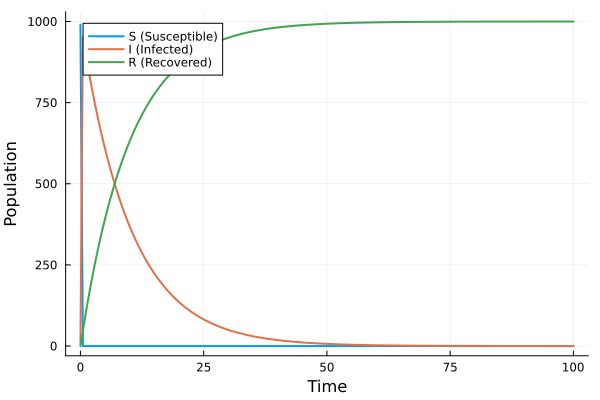
\includegraphics[width=0.7\textwidth,height=\textheight]{image/sir_det_dynamics.png}

}

\caption{\label{fig-003}Детерминистический график динамики SIR}

\end{figure}%

\begin{figure}

\centering{

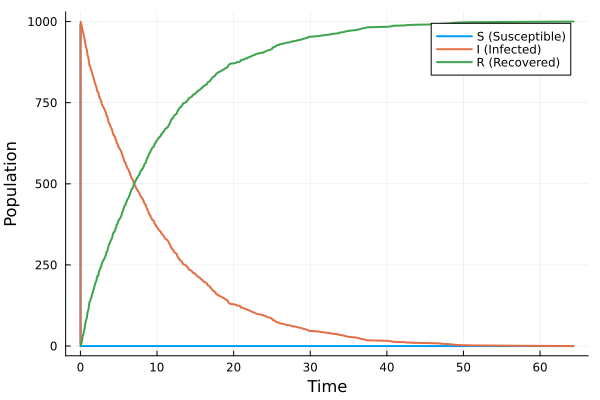
\includegraphics[width=0.7\textwidth,height=\textheight]{image/sir_stoch_dynamics.png}

}

\caption{\label{fig-004}Стохастический график динамики SIR}

\end{figure}%

Я генерировала файл jupyter, запускала все ячейке и все сработала без
ощибок(рис.5)

\begin{figure}

\centering{


\includegraphics[width=0.7\textwidth,height=\textheight]{image/pic3.png}

}

\caption{\label{fig-005}файл jupyter}

\end{figure}%

\textbf{\emph{Ниже приведен код, результаты расчетов и графики для кода
в файле scripts/sirpetri\_run.qmd}}

\section{Базовый прогон
модели}\label{ux431ux430ux437ux43eux432ux44bux439-ux43fux440ux43eux433ux43eux43d-ux43cux43eux434ux435ux43bux438-1}

\begin{Shaded}
\begin{Highlighting}[]
\ImportTok{using} \BuiltInTok{DrWatson}
\PreprocessorTok{@quickactivate} \StringTok{"project"}
\ImportTok{using} \BuiltInTok{Random}
\FunctionTok{include}\NormalTok{(}\FunctionTok{srcdir}\NormalTok{(}\StringTok{"SIRPetri.jl"}\NormalTok{))}
\ImportTok{using} \BuiltInTok{.SIRPetri}
\ImportTok{using} \BuiltInTok{DataFrames}\NormalTok{, }\BuiltInTok{CSV}\NormalTok{, }\BuiltInTok{Plots}
\end{Highlighting}
\end{Shaded}

\begin{verbatim}
┌ Warning: DrWatson could not find find a project file by recursively checking given `dir` and its parents. Returning `nothing` instead.
│ (given dir: /home/nelianjovu)
└ @ DrWatson ~/.julia/packages/DrWatson/2QF5p/src/project_setup.jl:84
WARNING: replacing module SIRPetri.
WARNING: using SIRPetri.build_sir_network in module Main conflicts with an existing identifier.
WARNING: using SIRPetri.simulate_deterministic in module Main conflicts with an existing identifier.
WARNING: using SIRPetri.simulate_stochastic in module Main conflicts with an existing identifier.
WARNING: using SIRPetri.plot_sir in module Main conflicts with an existing identifier.
\end{verbatim}

Выполняет один базовый эксперимент с фиксированными параметрами β = 0.3,
γ = 0.1.

Параметры

\begin{Shaded}
\begin{Highlighting}[]
\NormalTok{β }\OperatorTok{=} \FloatTok{0.3}
\NormalTok{γ }\OperatorTok{=} \FloatTok{0.1}
\NormalTok{tmax }\OperatorTok{=} \FloatTok{100.0}
\end{Highlighting}
\end{Shaded}

\begin{verbatim}
100.0
\end{verbatim}

Создаём сеть

\begin{Shaded}
\begin{Highlighting}[]
\NormalTok{net, u0, states }\OperatorTok{=} \FunctionTok{build\_sir\_network}\NormalTok{(β, γ)}
\end{Highlighting}
\end{Shaded}

\begin{verbatim}
(AlgebraicPetri.LabelledPetriNet:
  T = 1:2
  S = 1:3
  I = 1:3
  O = 1:3
  Name = 1:0
  it : I → T = [1, 1, 2]
  is : I → S = [1, 2, 2]
  ot : O → T = [1, 1, 2]
  os : O → S = [2, 2, 3]
  tname : T → Name = [:infection, :recovery]
  sname : S → Name = [:S, :I, :R], [990.0, 10.0, 0.0], [:S, :I, :R])
\end{verbatim}

\textbf{Запускает два типа симуляции}

детерминированную (решение ОДУ) --- даёт плавную усреднённую динамику;

\begin{Shaded}
\begin{Highlighting}[]
\NormalTok{df\_det }\OperatorTok{=} \FunctionTok{simulate\_deterministic}\NormalTok{(net, u0, (}\FloatTok{0.0}\NormalTok{, tmax), saveat }\OperatorTok{=} \FloatTok{0.5}\NormalTok{, rates }\OperatorTok{=}\NormalTok{ [β, γ])}
\end{Highlighting}
\end{Shaded}

\begin{tabular}{r|cccc}
    & time & S & I & R\\
    \hline
    & Float64 & Float64 & Float64 & Float64\\
    \hline
    1 & 0.0 & 990.0 & 10.0 & 0.0 \\
    2 & 0.5 & 2.47053e-7 & 952.691 & 47.3086 \\
    3 & 1.0 & 3.28252e-7 & 906.228 & 93.7719 \\
    4 & 1.5 & -1.78365e-7 & 862.031 & 137.969 \\
    5 & 2.0 & -2.6597e-7 & 819.989 & 180.011 \\
    6 & 2.5 & 2.389e-7 & 779.998 & 220.002 \\
    7 & 3.0 & -3.23518e-7 & 741.957 & 258.043 \\
    8 & 3.5 & -2.30682e-7 & 705.771 & 294.229 \\
    9 & 4.0 & 3.04028e-8 & 671.35 & 328.65 \\
    10 & 4.5 & 3.63345e-8 & 638.608 & 361.392 \\
    11 & 5.0 & -3.54734e-7 & 607.463 & 392.537 \\
    12 & 5.5 & -3.48967e-8 & 577.837 & 422.163 \\
    13 & 6.0 & 2.30028e-7 & 549.655 & 450.345 \\
    14 & 6.5 & 3.24586e-8 & 522.848 & 477.152 \\
    15 & 7.0 & -3.61058e-7 & 497.349 & 502.651 \\
    16 & 7.5 & -2.03624e-7 & 473.093 & 526.907 \\
    17 & 8.0 & 4.39154e-7 & 450.02 & 549.98 \\
    18 & 8.5 & 1.58379e-7 & 428.072 & 571.928 \\
    19 & 9.0 & -2.08057e-7 & 407.195 & 592.805 \\
    20 & 9.5 & -2.44636e-7 & 387.335 & 612.665 \\
    21 & 10.0 & 1.2209e-7 & 368.445 & 631.555 \\
    22 & 10.5 & 1.73937e-7 & 350.476 & 649.524 \\
    23 & 11.0 & 6.83511e-8 & 333.383 & 666.617 \\
    24 & 11.5 & -1.72158e-7 & 317.123 & 682.877 \\
    25 & 12.0 & 3.64045e-7 & 301.657 & 698.343 \\
    26 & 12.5 & -3.92833e-7 & 286.945 & 713.055 \\
    27 & 13.0 & -3.79316e-7 & 272.951 & 727.049 \\
    28 & 13.5 & 1.90957e-7 & 259.639 & 740.361 \\
    29 & 14.0 & -2.2568e-7 & 246.976 & 753.024 \\
    30 & 14.5 & 4.2444e-7 & 234.931 & 765.069 \\
    $\dots$ & $\dots$ & $\dots$ & $\dots$ & $\dots$ \\
\end{tabular}

стохастическую (алгоритм Гиллеспи) --- учитывает случайные флуктуации.

\begin{Shaded}
\begin{Highlighting}[]
\BuiltInTok{Random}\NormalTok{.}\FunctionTok{seed!}\NormalTok{(}\FloatTok{123}\NormalTok{)}
\NormalTok{df\_stoch }\OperatorTok{=} \FunctionTok{simulate\_stochastic}\NormalTok{(net, u0, (}\FloatTok{0.0}\NormalTok{, tmax), rates }\OperatorTok{=}\NormalTok{ [β, γ])}
\end{Highlighting}
\end{Shaded}

\begin{tabular}{r|cccc}
    & time & S & I & R\\
    \hline
    & Float64 & Float64 & Float64 & Float64\\
    \hline
    1 & 0.0 & 990.0 & 10.0 & 0.0 \\
    2 & 0.000219318 & 989.0 & 11.0 & 0.0 \\
    3 & 0.00025471 & 988.0 & 12.0 & 0.0 \\
    4 & 0.000435457 & 987.0 & 13.0 & 0.0 \\
    5 & 0.00124186 & 986.0 & 14.0 & 0.0 \\
    6 & 0.00137312 & 985.0 & 15.0 & 0.0 \\
    7 & 0.00151759 & 984.0 & 16.0 & 0.0 \\
    8 & 0.00219412 & 983.0 & 17.0 & 0.0 \\
    9 & 0.00239638 & 982.0 & 18.0 & 0.0 \\
    10 & 0.00245828 & 981.0 & 19.0 & 0.0 \\
    11 & 0.00253136 & 980.0 & 20.0 & 0.0 \\
    12 & 0.00274985 & 979.0 & 21.0 & 0.0 \\
    13 & 0.00277041 & 978.0 & 22.0 & 0.0 \\
    14 & 0.00291987 & 977.0 & 23.0 & 0.0 \\
    15 & 0.00327978 & 976.0 & 24.0 & 0.0 \\
    16 & 0.00338914 & 975.0 & 25.0 & 0.0 \\
    17 & 0.00360517 & 974.0 & 26.0 & 0.0 \\
    18 & 0.00367641 & 973.0 & 27.0 & 0.0 \\
    19 & 0.00394413 & 972.0 & 28.0 & 0.0 \\
    20 & 0.00406046 & 971.0 & 29.0 & 0.0 \\
    21 & 0.00437152 & 970.0 & 30.0 & 0.0 \\
    22 & 0.00448011 & 969.0 & 31.0 & 0.0 \\
    23 & 0.00458821 & 968.0 & 32.0 & 0.0 \\
    24 & 0.00473125 & 967.0 & 33.0 & 0.0 \\
    25 & 0.00474643 & 966.0 & 34.0 & 0.0 \\
    26 & 0.00497684 & 965.0 & 35.0 & 0.0 \\
    27 & 0.0049977 & 964.0 & 36.0 & 0.0 \\
    28 & 0.00501235 & 963.0 & 37.0 & 0.0 \\
    29 & 0.00504887 & 962.0 & 38.0 & 0.0 \\
    30 & 0.00508054 & 961.0 & 39.0 & 0.0 \\
    $\dots$ & $\dots$ & $\dots$ & $\dots$ & $\dots$ \\
\end{tabular}

Сохраняет результаты в CSV‑файлы и строит графики S(t), I(t), R(t) для
обоих типов.

\begin{Shaded}
\begin{Highlighting}[]
\NormalTok{CSV.}\FunctionTok{write}\NormalTok{(}\FunctionTok{datadir}\NormalTok{(}\StringTok{"sir\_det.csv"}\NormalTok{), df\_det)}
\NormalTok{CSV.}\FunctionTok{write}\NormalTok{(}\FunctionTok{datadir}\NormalTok{(}\StringTok{"sir\_stoch.csv"}\NormalTok{), df\_stoch)}
\end{Highlighting}
\end{Shaded}

\begin{verbatim}
"/home/nelianjovu/work/study/2026-1/2026-1==study--simulationmod/2026-1--study--simulationmod/labs/lab06/project/data/sir_stoch.csv"
\end{verbatim}

Графики

\begin{Shaded}
\begin{Highlighting}[]
\NormalTok{p\_det }\OperatorTok{=} \FunctionTok{plot\_sir}\NormalTok{(df\_det)}
\FunctionTok{savefig}\NormalTok{(}\FunctionTok{plotsdir}\NormalTok{(}\StringTok{"sir\_det\_dynamics.png"}\NormalTok{))}

\NormalTok{p\_stoch }\OperatorTok{=} \FunctionTok{plot\_sir}\NormalTok{(df\_stoch)}
\FunctionTok{savefig}\NormalTok{(}\FunctionTok{plotsdir}\NormalTok{(}\StringTok{"sir\_stoch\_dynamics.png"}\NormalTok{))}

\FunctionTok{println}\NormalTok{(}\StringTok{"Базовый прогон завершён. Результаты в data/ и plots/"}\NormalTok{)}
\end{Highlighting}
\end{Shaded}

\begin{verbatim}
Базовый прогон завершён. Результаты в data/ и plots/
\end{verbatim}

Я добавила несколько параметров, чтобы посмотреть, как будет выглядеть
график(рис.6)

\begin{figure}

\centering{


\includegraphics[width=0.7\textwidth,height=\textheight]{image/pic4.png}

}

\caption{\label{fig-006}Скрипт базового эксперимент(с параметром)}

\end{figure}%

Для обе типы симуляции, ничего сильно меняется, просто время пика(рис.7,
8, 9, 10, 11, 12)

\begin{figure}

\centering{

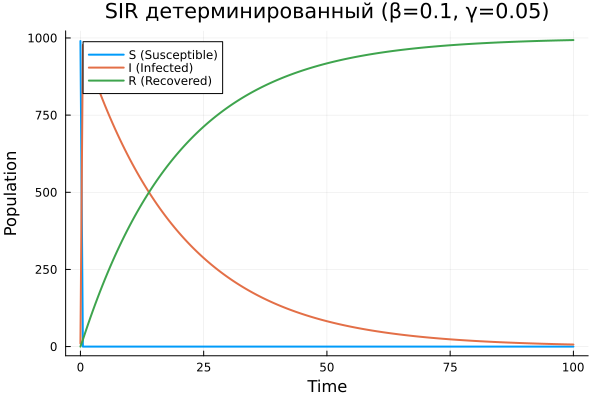
\includegraphics[width=0.7\textwidth,height=\textheight]{image/sir_det_dynamics_0.png}

}

\caption{\label{fig-007}Детерминистический график динамики SIR}

\end{figure}%

\begin{figure}

\centering{

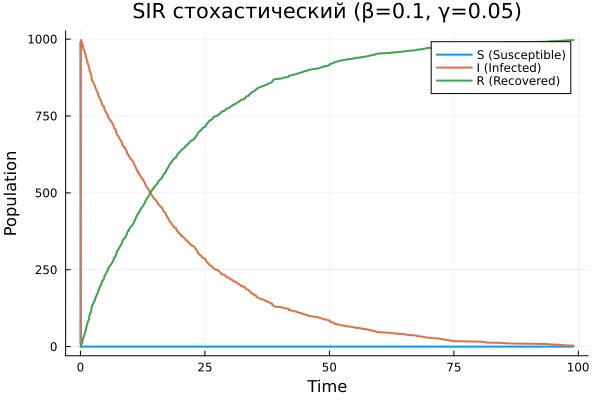
\includegraphics[width=0.7\textwidth,height=\textheight]{image/sir_stoch_dynamics_0.png}

}

\caption{\label{fig-008}Стохастический график динамики SIR}

\end{figure}%

\begin{figure}

\centering{

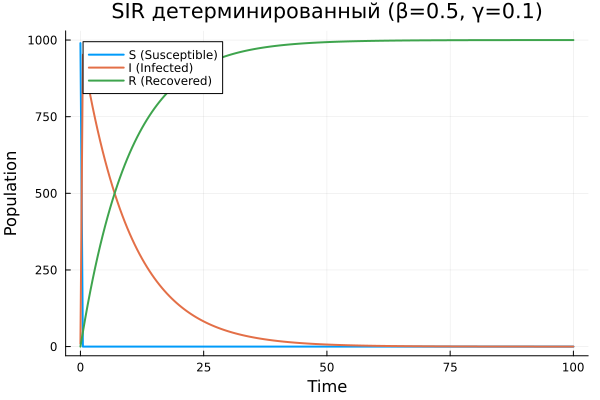
\includegraphics[width=0.7\textwidth,height=\textheight]{image/sir_det_dynamics_1.png}

}

\caption{\label{fig-009}Детерминистический график динамики SIR}

\end{figure}%

\begin{figure}

\centering{

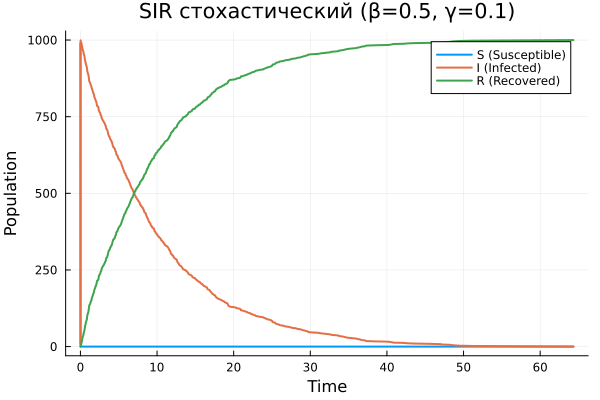
\includegraphics[width=0.7\textwidth,height=\textheight]{image/sir_stoch_dynamics_1.png}

}

\caption{\label{fig-010}Стохастический график динамики SIR}

\end{figure}%

\begin{figure}

\centering{

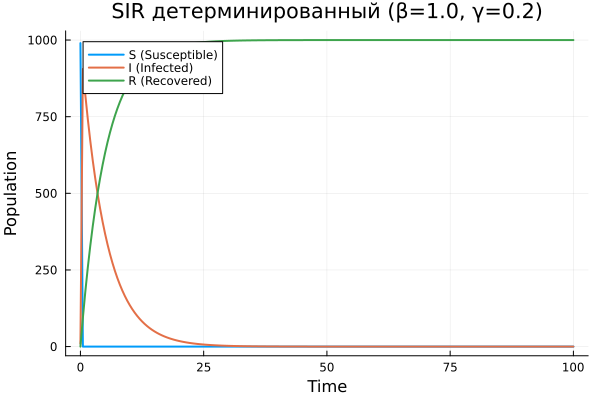
\includegraphics[width=0.7\textwidth,height=\textheight]{image/sir_det_dynamics_2.png}

}

\caption{\label{fig-011}Детерминистический график динамики SIR}

\end{figure}%

\begin{figure}

\centering{

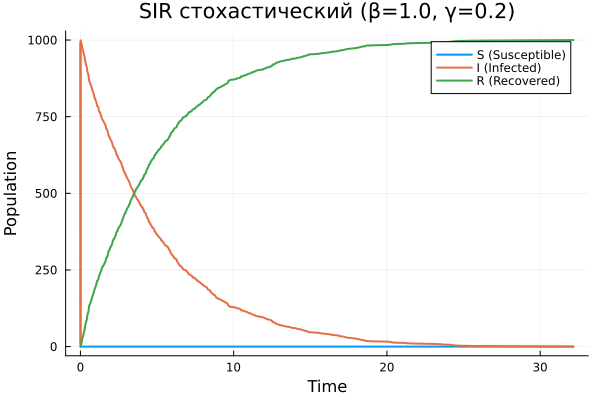
\includegraphics[width=0.7\textwidth,height=\textheight]{image/sir_stoch_dynamics_2.png}

}

\caption{\label{fig-012}Стохастический график динамики SIR}

\end{figure}%

Я генерировала файл jupyter, запускала все ячейке и все сработала без
ощибок(рис.13)

\begin{figure}

\centering{


\includegraphics[width=0.7\textwidth,height=\textheight]{image/pic5.png}

}

\caption{\label{fig-013}файл jupyter}

\end{figure}%

\textbf{\emph{Ниже приведен код, результаты расчетов и графики для кода
в файле scripts/sirpetri\_run\_param.qmd}}

\section{Базовый прогон модели SIR (Petri
nets)}\label{ux431ux430ux437ux43eux432ux44bux439-ux43fux440ux43eux433ux43eux43d-ux43cux43eux434ux435ux43bux438-sir-petri-nets}

\begin{Shaded}
\begin{Highlighting}[]
\ImportTok{using} \BuiltInTok{DrWatson}
\PreprocessorTok{@quickactivate} \StringTok{"project"}
\ImportTok{using} \BuiltInTok{Random}
\FunctionTok{include}\NormalTok{(}\FunctionTok{srcdir}\NormalTok{(}\StringTok{"SIRPetri.jl"}\NormalTok{))}
\ImportTok{using} \BuiltInTok{.SIRPetri}
\ImportTok{using} \BuiltInTok{DataFrames}\NormalTok{, }\BuiltInTok{CSV}\NormalTok{, }\BuiltInTok{Plots}
\end{Highlighting}
\end{Shaded}

\begin{verbatim}
┌ Warning: DrWatson could not find find a project file by recursively checking given `dir` and its parents. Returning `nothing` instead.
│ (given dir: /home/nelianjovu)
└ @ DrWatson ~/.julia/packages/DrWatson/2QF5p/src/project_setup.jl:84
WARNING: replacing module SIRPetri.
WARNING: using SIRPetri.build_sir_network in module Main conflicts with an existing identifier.
WARNING: using SIRPetri.simulate_deterministic in module Main conflicts with an existing identifier.
WARNING: using SIRPetri.simulate_stochastic in module Main conflicts with an existing identifier.
WARNING: using SIRPetri.plot_sir in module Main conflicts with an existing identifier.
\end{verbatim}

Выполняет базовые эксперименты с разными параметрами β и γ.

Параметры для трёх экспериментов

\begin{Shaded}
\begin{Highlighting}[]
\NormalTok{experiments }\OperatorTok{=}\NormalTok{ [}
\NormalTok{    (β }\OperatorTok{=} \FloatTok{0.1}\NormalTok{, γ }\OperatorTok{=} \FloatTok{0.05}\NormalTok{, name }\OperatorTok{=} \StringTok{"0"}\NormalTok{),}
\NormalTok{    (β }\OperatorTok{=} \FloatTok{0.5}\NormalTok{, γ }\OperatorTok{=} \FloatTok{0.1}\NormalTok{, name }\OperatorTok{=} \StringTok{"1"}\NormalTok{),}
\NormalTok{    (β }\OperatorTok{=} \FloatTok{1.0}\NormalTok{, γ }\OperatorTok{=} \FloatTok{0.2}\NormalTok{, name }\OperatorTok{=} \StringTok{"2"}\NormalTok{)}
\NormalTok{]}

\NormalTok{tmax }\OperatorTok{=} \FloatTok{100.0}
\end{Highlighting}
\end{Shaded}

\begin{verbatim}
100.0
\end{verbatim}

\begin{Shaded}
\begin{Highlighting}[]
\ControlFlowTok{for}\NormalTok{ exp }\KeywordTok{in}\NormalTok{ experiments}
\NormalTok{    β, γ, name }\OperatorTok{=}\NormalTok{ exp.β, exp.γ, exp.name}
    \FunctionTok{println}\NormalTok{(}\StringTok{"}\SpecialCharTok{\textbackslash{}n}\StringTok{Эксперимент }\SpecialCharTok{$}\NormalTok{name}\StringTok{: β = }\SpecialCharTok{$}\StringTok{β, γ = }\SpecialCharTok{$}\StringTok{γ, }\NormalTok{R}\StringTok{₀ = }\SpecialCharTok{$}\NormalTok{(β}\OperatorTok{/}\NormalTok{γ)}\StringTok{"}\NormalTok{)}
\NormalTok{    net, u0, states }\OperatorTok{=} \FunctionTok{build\_sir\_network}\NormalTok{(β, γ) }\CommentTok{\# Создаём сеть Петри для SIR модели}

\NormalTok{    df\_det }\OperatorTok{=} \FunctionTok{simulate\_deterministic}\NormalTok{(}
\NormalTok{        net, u0, (}\FloatTok{0.0}\NormalTok{, tmax),}
\NormalTok{        saveat }\OperatorTok{=} \FloatTok{0.5}\NormalTok{,}
\NormalTok{        rates }\OperatorTok{=}\NormalTok{ [β, γ]}
\NormalTok{    )}\CommentTok{\# Детерминированная симуляция (решение ОДУ)}

    \BuiltInTok{Random}\NormalTok{.}\FunctionTok{seed!}\NormalTok{(}\FloatTok{123}\NormalTok{)}
\NormalTok{    df\_stoch }\OperatorTok{=} \FunctionTok{simulate\_stochastic}\NormalTok{(}
\NormalTok{        net, u0, (}\FloatTok{0.0}\NormalTok{, tmax),}
\NormalTok{        rates }\OperatorTok{=}\NormalTok{ [β, γ]}
\NormalTok{    )}\CommentTok{\# Стохастическая симуляция (алгоритм Гиллеспи)}

\NormalTok{    CSV.}\FunctionTok{write}\NormalTok{(}\FunctionTok{datadir}\NormalTok{(}\StringTok{"sir\_det\_}\SpecialCharTok{$}\NormalTok{name}\StringTok{.csv"}\NormalTok{), df\_det)}
\NormalTok{    CSV.}\FunctionTok{write}\NormalTok{(}\FunctionTok{datadir}\NormalTok{(}\StringTok{"sir\_stoch\_}\SpecialCharTok{$}\NormalTok{name}\StringTok{.csv"}\NormalTok{), df\_stoch)}

\NormalTok{    p\_det }\OperatorTok{=} \FunctionTok{plot\_sir}\NormalTok{(df\_det) }\CommentTok{\# Строим и сохраняем графики}
    \FunctionTok{title!}\NormalTok{(p\_det, }\StringTok{"SIR детерминированный (β=}\SpecialCharTok{$}\StringTok{β, γ=}\SpecialCharTok{$}\StringTok{γ)")}
\StringTok{    }\NormalTok{savefig}\StringTok{(plotsdir("}\NormalTok{sir\_det\_dynamics\_}\OperatorTok{$}\NormalTok{name.png}\StringTok{"))}

\NormalTok{    p\_stoch }\OperatorTok{=} \FunctionTok{plot\_sir}\NormalTok{(df\_stoch)}
    \FunctionTok{title!}\NormalTok{(p\_stoch, }\StringTok{"SIR стохастический (β=}\SpecialCharTok{$}\StringTok{β, γ=}\SpecialCharTok{$}\StringTok{γ)")}
\StringTok{    }\NormalTok{savefig}\StringTok{(plotsdir("}\NormalTok{sir\_stoch\_dynamics\_}\OperatorTok{$}\NormalTok{name.png}\StringTok{"))}

\ControlFlowTok{end}

\FunctionTok{println}\NormalTok{(}\StringTok{"}\SpecialCharTok{\textbackslash{}n}\StringTok{Базовый прогон завершён. Результаты в data/ и plots/"}\NormalTok{)}
\end{Highlighting}
\end{Shaded}

\begin{verbatim}

Эксперимент 0: β = 0.1, γ = 0.05, R₀ = 2.0

Эксперимент 1: β = 0.5, γ = 0.1, R₀ = 5.0

Эксперимент 2: β = 1.0, γ = 0.2, R₀ = 5.0

Базовый прогон завершён. Результаты в data/ и plots/
\end{verbatim}

\section{\texorpdfstring{3. Коэффициент заражения
\(\beta\)}{3. Коэффициент заражения \textbackslash beta}}\label{ux43aux43eux44dux444ux444ux438ux446ux438ux435ux43dux442-ux437ux430ux440ux430ux436ux435ux43dux438ux44f-beta}

Я создала фаий scripts/sirpetri\_scan\_parameters.jl и скопировала
заданный скрипт в него. Скрипт Исследуется чувствительность модели к
изменению параметра \(\beta\) (скорости заражения). Для каждого значения
\(\beta\) из диапазона 0.1:0.05:0.8 запускается детерминированная
симуляция (γ = 0.1 фиксирован) и вычисляются: максимальное число
инфицированных (пик эпидемии) -- peak\_I и конечное число выздоровевших
-- final\_R. Я преобразовала скрипт в литератуный стиль и запускала
его(рис.14)

\begin{figure}

\centering{


\includegraphics[width=0.7\textwidth,height=\textheight]{image/pic6.png}

}

\caption{\label{fig-014}Скрипт коэффициента заражения \(\beta\)}

\end{figure}%

После запуск, получила график. На графике показано, что при всех
тестируемых значениях \(\beta\) инфекция распространяется почти по всей
популяции, что соответствует конечному значению R ≈ N. В результате в
этом моделировании не наблюдается порогового значения. Пиковое число
инфицированных индивидуумов изменяется незначительно при изменении
\(\beta\)(рис 15)

\begin{figure}

\centering{

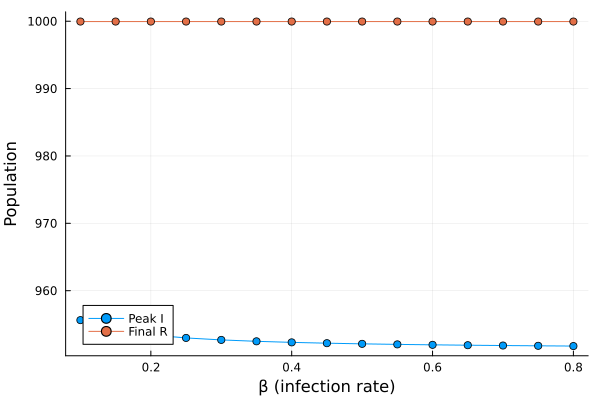
\includegraphics[width=0.7\textwidth,height=\textheight]{image/sir_scan.png}

}

\caption{\label{fig-015}Коэффициент заражения \(\beta\)}

\end{figure}%

Я генерировала файл jupyter, запускала все ячейке и все сработала без
ощибок(рис.16)

\begin{figure}

\centering{


\includegraphics[width=0.7\textwidth,height=\textheight]{image/pic7.png}

}

\caption{\label{fig-016}файл jupyter}

\end{figure}%

\textbf{\emph{Ниже приведен код, результаты расчетов и графики для кода
в файле scripts/sirpetri\_scan\_parameters.qmd}}

\section{Коэффициент заражения
β}\label{ux43aux43eux44dux444ux444ux438ux446ux438ux435ux43dux442-ux437ux430ux440ux430ux436ux435ux43dux438ux44f-ux3b2}

\begin{Shaded}
\begin{Highlighting}[]
\ImportTok{using} \BuiltInTok{DrWatson}
\PreprocessorTok{@quickactivate} \StringTok{"project"}
\FunctionTok{include}\NormalTok{(}\FunctionTok{srcdir}\NormalTok{(}\StringTok{"SIRPetri.jl"}\NormalTok{))}
\ImportTok{using} \BuiltInTok{.SIRPetri}
\ImportTok{using} \BuiltInTok{DataFrames}\NormalTok{, }\BuiltInTok{CSV}\NormalTok{, }\BuiltInTok{Plots}
\end{Highlighting}
\end{Shaded}

\begin{verbatim}
┌ Warning: DrWatson could not find find a project file by recursively checking given `dir` and its parents. Returning `nothing` instead.
│ (given dir: /home/nelianjovu)
└ @ DrWatson ~/.julia/packages/DrWatson/2QF5p/src/project_setup.jl:84
WARNING: replacing module SIRPetri.
WARNING: using SIRPetri.build_sir_network in module Main conflicts with an existing identifier.
WARNING: using SIRPetri.simulate_deterministic in module Main conflicts with an existing identifier.
WARNING: using SIRPetri.simulate_stochastic in module Main conflicts with an existing identifier.
WARNING: using SIRPetri.plot_sir in module Main conflicts with an existing identifier.
\end{verbatim}

Исследуется чувствительность модели к изменению параметра β (скорости
заражения)

\begin{Shaded}
\begin{Highlighting}[]
\NormalTok{β\_range }\OperatorTok{=} \FloatTok{0.1}\OperatorTok{:}\FloatTok{0.05}\OperatorTok{:}\FloatTok{0.8}
\NormalTok{γ\_fixed }\OperatorTok{=} \FloatTok{0.1}
\NormalTok{tmax }\OperatorTok{=} \FloatTok{100.0}

\NormalTok{results }\OperatorTok{=}\NormalTok{ []}
\end{Highlighting}
\end{Shaded}

\begin{verbatim}
Any[]
\end{verbatim}

Для каждого значения β из диапазона 0.1:0.05:0.8 запускается
детерминированная симуляция (γ = 0.1 фиксирован)

Для каждого прогона вычисляются:

\begin{enumerate}
\def\labelenumi{\arabic{enumi}.}
\item
  максимальное число инфицированных (пик эпидемии) -- peak\_I;
\item
  конечное число выздоровевших -- final\_R.
\end{enumerate}

\begin{Shaded}
\begin{Highlighting}[]
\ControlFlowTok{for}\NormalTok{ β }\KeywordTok{in}\NormalTok{ β\_range}
\NormalTok{    net, u0, \_ }\OperatorTok{=} \FunctionTok{build\_sir\_network}\NormalTok{(β, γ\_fixed)}
\NormalTok{    df }\OperatorTok{=} \FunctionTok{simulate\_deterministic}\NormalTok{(net, u0, (}\FloatTok{0.0}\NormalTok{, tmax), saveat }\OperatorTok{=} \FloatTok{0.5}\NormalTok{, rates }\OperatorTok{=}\NormalTok{ [β, γ\_fixed])}
\NormalTok{    peak\_I }\OperatorTok{=} \FunctionTok{maximum}\NormalTok{(df.I)}
\NormalTok{    final\_R }\OperatorTok{=}\NormalTok{ df.R[}\KeywordTok{end}\NormalTok{]}
    \FunctionTok{push!}\NormalTok{(results, (β }\OperatorTok{=}\NormalTok{ β, peak\_I }\OperatorTok{=}\NormalTok{ peak\_I, final\_R }\OperatorTok{=}\NormalTok{ final\_R))}
\ControlFlowTok{end}
\end{Highlighting}
\end{Shaded}

Результаты сводятся в таблицу и строится график зависимости peak\_I(β) и
final\_R(β

\begin{Shaded}
\begin{Highlighting}[]
\NormalTok{df\_scan }\OperatorTok{=} \FunctionTok{DataFrame}\NormalTok{(results)}
\NormalTok{CSV.}\FunctionTok{write}\NormalTok{(}\FunctionTok{datadir}\NormalTok{(}\StringTok{"sir\_scan.csv"}\NormalTok{), df\_scan)}
\end{Highlighting}
\end{Shaded}

\begin{verbatim}
"/home/nelianjovu/work/study/2026-1/2026-1==study--simulationmod/2026-1--study--simulationmod/labs/lab06/project/data/sir_scan.csv"
\end{verbatim}

График

\begin{Shaded}
\begin{Highlighting}[]
\NormalTok{p }\OperatorTok{=} \FunctionTok{plot}\NormalTok{(}
\NormalTok{    df\_scan.β,}
\NormalTok{    [df\_scan.peak\_I df\_scan.final\_R],}
\NormalTok{    label }\OperatorTok{=}\NormalTok{ [}\StringTok{"Peak I"} \StringTok{"Final R"}\NormalTok{],}
\NormalTok{    marker }\OperatorTok{=} \OperatorTok{:}\NormalTok{circle,}
\NormalTok{    xlabel }\OperatorTok{=} \StringTok{"β (infection rate)"}\NormalTok{,}
\NormalTok{    ylabel }\OperatorTok{=} \StringTok{"Population"}\NormalTok{,}
\NormalTok{    )}
\FunctionTok{savefig}\NormalTok{(}\FunctionTok{plotsdir}\NormalTok{(}\StringTok{"sir\_scan.png"}\NormalTok{))}

\FunctionTok{println}\NormalTok{(}\StringTok{"Сканирование β завершено. Результат в data/sir\_scan.csv"}\NormalTok{)}
\end{Highlighting}
\end{Shaded}

\begin{verbatim}
Сканирование β завершено. Результат в data/sir_scan.csv
\end{verbatim}

\section{4. Анимация детерминированной
динамики}\label{ux430ux43dux438ux43cux430ux446ux438ux44f-ux434ux435ux442ux435ux440ux43cux438ux43dux438ux440ux43eux432ux430ux43dux43dux43eux439-ux434ux438ux43dux430ux43cux438ux43aux438}

Я создала фаий scripts/sirpetri\_animate.jl и писала скрипт в него.
Скрипт создаёт GIF-анимацию, показывающую, как со временем меняется
количество людей в каждой из трёх групп (S, I, R). Анимация позволяет
наглядно увидеть распространение эпидемии, пик и спад.(рис.17)

\begin{figure}

\centering{


\includegraphics[width=0.7\textwidth,height=\textheight]{image/pic8.png}

}

\caption{\label{fig-017}Скрипт анимации}

\end{figure}%

После запуск, получила GIF. В момент времени t = 0 популяция почти
полностью восприимчива, имеется лишь небольшое число инфицированных и ни
одного выздоровевшего человека. Это представляет собой начальную стадию
распространения болезни, с которой развивается эпидемия.

\section{5. Итоговый
отчёт}\label{ux438ux442ux43eux433ux43eux432ux44bux439-ux43eux442ux447ux451ux442}

Я создала фаий scripts/sirpetri\_report.jl и скопировала заданный скрипт
в него. Скрипт загружает ранее сохранённые результаты (sir\_det.csv,
sir\_stoch.csv, sir\_scan.csv) и строит сравнительные графики для
итогового отчёта: Сравнение детерминированной и стохастической динамики
инфицированных I(t) и зависимость пика I от β (результат сканирования).
Я преобразовала скрипт в литератуный стиль и запускала его(рис.18)

\begin{figure}

\centering{


\includegraphics[width=0.7\textwidth,height=\textheight]{image/pic9.png}

}

\caption{\label{fig-018}Скрипт итогового отчёта}

\end{figure}%

После запуск, получила два графики. Сравнение детерминированной и
стохастической кривых I(t) показывает, насколько велик разброс,
вызванный случайностью. При большом размере популяции они близки. График
чувствительности позволяет количественно оценить, как изменение
заразности β влияет на тяжесть эпидемии (пик I). Это важно для принятия
решений (например, меры по снижению β)(рис 19 и 20)

\begin{figure}

\centering{

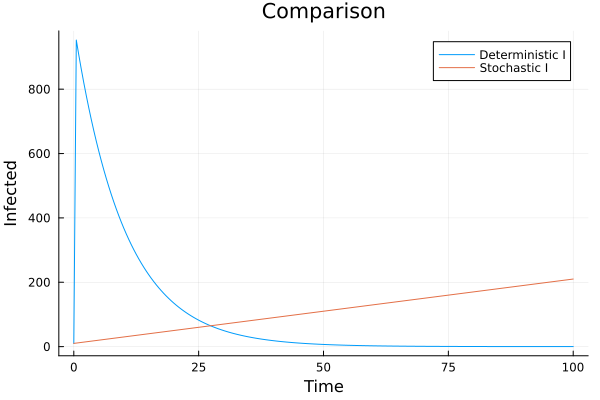
\includegraphics[width=0.7\textwidth,height=\textheight]{image/comparison.png}

}

\caption{\label{fig-019}Детерминированный и стохастический графики}

\end{figure}%

\begin{figure}

\centering{

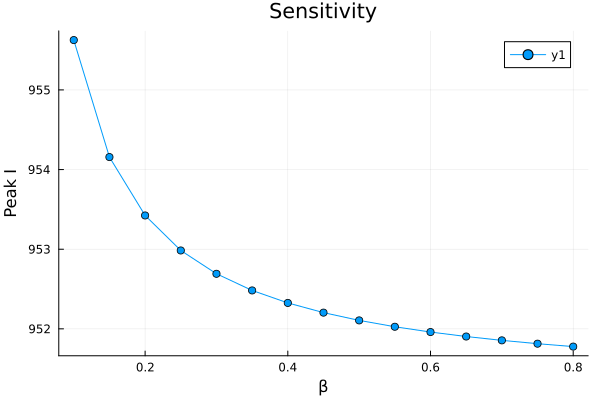
\includegraphics[width=0.7\textwidth,height=\textheight]{image/sensitivity.png}

}

\caption{\label{fig-020}Зависимость пика I от \beta}

\end{figure}%

Я генерировала файл jupyter, запускала все ячейке и все сработала без
ощибок(рис.21)

\begin{figure}

\centering{


\includegraphics[width=0.7\textwidth,height=\textheight]{image/pic10.png}

}

\caption{\label{fig-021}файл jupyter}

\end{figure}%

\textbf{\emph{Ниже приведен код, результаты расчетов и графики для кода
в файле scripts/sirpetri\_report.qmd}}

\section{Итоговый
отчёт}\label{ux438ux442ux43eux433ux43eux432ux44bux439-ux43eux442ux447ux451ux442-1}

\begin{Shaded}
\begin{Highlighting}[]
\ImportTok{using} \BuiltInTok{DrWatson}
\PreprocessorTok{@quickactivate} \StringTok{"project"}
\ImportTok{using} \BuiltInTok{DataFrames}\NormalTok{, }\BuiltInTok{CSV}\NormalTok{, }\BuiltInTok{Plots}
\end{Highlighting}
\end{Shaded}

\begin{verbatim}
┌ Warning: DrWatson could not find find a project file by recursively checking given `dir` and its parents. Returning `nothing` instead.
│ (given dir: /home/nelianjovu)
└ @ DrWatson ~/.julia/packages/DrWatson/2QF5p/src/project_setup.jl:84
\end{verbatim}

Загружает ранее сохранённые результаты (sir\_det.csv, sir\_stoch.csv,
sir\_scan.csv) и строит сравнительные графики для итогового отчёта: 1.
Сравнение детерминированной и стохастической динамики инфицированных
I(t). 2. Зависимость пика I от β (результат сканирования).

\begin{Shaded}
\begin{Highlighting}[]
\NormalTok{df\_det }\OperatorTok{=}\NormalTok{ CSV.}\FunctionTok{read}\NormalTok{(}\FunctionTok{datadir}\NormalTok{(}\StringTok{"sir\_det.csv"}\NormalTok{), DataFrame)}
\NormalTok{df\_stoch }\OperatorTok{=}\NormalTok{ CSV.}\FunctionTok{read}\NormalTok{(}\FunctionTok{datadir}\NormalTok{(}\StringTok{"sir\_stoch.csv"}\NormalTok{), DataFrame)}
\NormalTok{df\_scan }\OperatorTok{=}\NormalTok{ CSV.}\FunctionTok{read}\NormalTok{(}\FunctionTok{datadir}\NormalTok{(}\StringTok{"sir\_scan.csv"}\NormalTok{), DataFrame)}
\end{Highlighting}
\end{Shaded}

\begin{tabular}{r|ccc}
    & β & peak\_I & final\_R\\
    \hline
    & Float64 & Float64 & Float64\\
    \hline
    1 & 0.1 & 955.626 & 999.954 \\
    2 & 0.15 & 954.157 & 999.954 \\
    3 & 0.2 & 953.424 & 999.954 \\
    4 & 0.25 & 952.984 & 999.955 \\
    5 & 0.3 & 952.691 & 999.955 \\
    6 & 0.35 & 952.482 & 999.955 \\
    7 & 0.4 & 952.326 & 999.955 \\
    8 & 0.45 & 952.204 & 999.955 \\
    9 & 0.5 & 952.106 & 999.955 \\
    10 & 0.55 & 952.026 & 999.955 \\
    11 & 0.6 & 951.96 & 999.955 \\
    12 & 0.65 & 951.904 & 999.955 \\
    13 & 0.7 & 951.856 & 999.955 \\
    14 & 0.75 & 951.814 & 999.955 \\
    15 & 0.8 & 951.777 & 999.955 \\
\end{tabular}

Сравнение детерминированной и стохастической динамики

\begin{Shaded}
\begin{Highlighting}[]
\NormalTok{p1 }\OperatorTok{=} \FunctionTok{plot}\NormalTok{(}
\NormalTok{    df\_det.time,}
\NormalTok{    [df\_det.I df\_stoch.I[}\FloatTok{1}\OperatorTok{:}\FunctionTok{length}\NormalTok{(df\_det.time)]],}
\NormalTok{    label }\OperatorTok{=}\NormalTok{ [}\StringTok{"Deterministic I"} \StringTok{"Stochastic I"}\NormalTok{],}
\NormalTok{    xlabel }\OperatorTok{=} \StringTok{"Time"}\NormalTok{,}
\NormalTok{    ylabel }\OperatorTok{=} \StringTok{"Infected"}\NormalTok{,}
\NormalTok{    title }\OperatorTok{=} \StringTok{"Comparison"}\NormalTok{,}
\NormalTok{    )}
\FunctionTok{savefig}\NormalTok{(}\FunctionTok{plotsdir}\NormalTok{(}\StringTok{"comparison.png"}\NormalTok{))}
\end{Highlighting}
\end{Shaded}

\begin{verbatim}
"/home/nelianjovu/work/study/2026-1/2026-1==study--simulationmod/2026-1--study--simulationmod/labs/lab06/project/plots/comparison.png"
\end{verbatim}

Зависимость пика I от β

\begin{Shaded}
\begin{Highlighting}[]
\NormalTok{p2 }\OperatorTok{=} \FunctionTok{plot}\NormalTok{(}
\NormalTok{    df\_scan.β,}
\NormalTok{    df\_scan.peak\_I,}
\NormalTok{    marker }\OperatorTok{=} \OperatorTok{:}\NormalTok{circle,}
\NormalTok{    xlabel }\OperatorTok{=} \StringTok{"β"}\NormalTok{,}
\NormalTok{    ylabel }\OperatorTok{=} \StringTok{"Peak I"}\NormalTok{,}
\NormalTok{    title }\OperatorTok{=} \StringTok{"Sensitivity"}\NormalTok{,}
\NormalTok{    )}
\FunctionTok{savefig}\NormalTok{(}\FunctionTok{plotsdir}\NormalTok{(}\StringTok{"sensitivity.png"}\NormalTok{))}

\FunctionTok{println}\NormalTok{(}\StringTok{"Отчётные графики сохранены в plots/"}\NormalTok{)}
\end{Highlighting}
\end{Shaded}

\begin{verbatim}
Отчётные графики сохранены в plots/
\end{verbatim}

\chapter{Выводы}\label{ux432ux44bux432ux43eux434ux44b}

В этой лабораторной работы, реализовали основные модели(модель SIR) в
подходе сетей Петри.


\printbibliography


\end{document}
